\chapter{RESULTADOS E DISCUSSÃO}
Este capítulo detalha os resultados alcançados por meio da simulação computacional do método de controle de trajetória proposto pelo presente trabalho. É apresentado a sequência de movimentos a serem simulados, assim como os valores das variáveis do método. Além disso, são realizadas simulações com variações dos parâmetros do método para uma análise da influência dos mesmos nos resultados. É utilizado também o algoritmo Runge-Kutta para simular a trajetória percorrida pela ponta da impressora dada a trajetória da base, fornecendo dados para se comparar a influência do método de controle de trajetória proposto.

\section{Simulação Computacional e Análise de Dados}

As simulações são realizadas a partir de dois movimentos lineares: um deslocamento de 10 milímetros no eixo x seguido de um movimento similar no eixo y, partindo da posição inicial (0,0) e em estado de repouso. A Figura \ref{fig:base_mov} ilustra estes movimentos.

\begin{figure}[H]
    \centering
    \caption{Movimento base}
    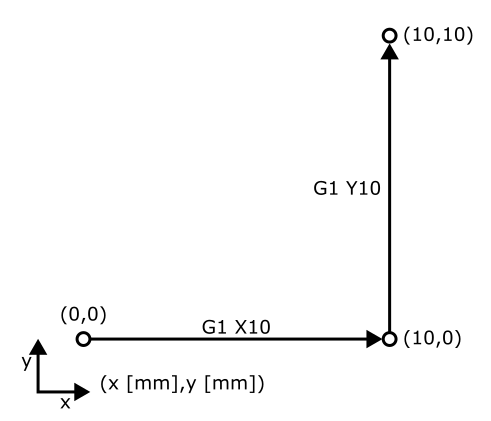
\includegraphics[scale=0.6]{base_mov}

    \label{fig:base_mov}
\end{figure}

\subsection{Simulação de Referência} 
É realizado uma simulação de referência com valores intermediários para servir de base de comparação para as simulações que variam os valores dos parâmetros. Os valores de referência dos parâmetros são apresentados na Tabela \ref{tab:base_params}.

\begin{table}
    \begin{center}
    \caption{Valores dos parâmetros utilizados na simulação referência.}
    \label{tab:base_params}
    \begin{tabular}{c c c}
        Parâmetro & Valor & Unidade\\ \hline
        Frequência & 100 & $rad/s$\\
        Coeficiente de amortecimento & 0,5 & - \\
        Aceleração base & 5000 & $mm/s^2$ \\
        Passo de tempo & 0,01 & $s$ \\ 
        Velocidade desejada & 100 & $mm/s$ \\ \hline
    \end{tabular}
    \end{center}
\end{table}

\subsection{Simulações com Parâmetros Variados}
A sequência de simulações das variações da frequência natural, do coeficiente de amortecimento, da aceleração de entrada, do passo de tempo e da velocidade desejada é construída a partir de valores inferiores e superiores aos valores da simulação de referência, alterando um parâmetro de cada vez, totalizando 11 simulações, sendo 10 destas simulações dos valores inferiores e superiores de cada um dos parâmetros e 1 simulação de referência utilizando os valores intermediários. %¨rodar o GPT aqui

Os valores das simulações é apresentado na Tabela \ref{tab:sim_params}. Onde cada simulação é identificada por um número, que indica qual parâmetro está sendo alterado, e uma letra, que indica o parâmetro modificado, sendo A para os valores inferiores e B para os valores superiores. %GPT aqui também

(ALTERAR OS VALORES DA TABELA)%deve estar ok

\begin{table}
    \begin{center}
    \caption{Parâmetros utilizados nas simulações.}
    \label{tab:sim_params}
    \begin{tabular}{c c c c c}
        Caso & Parâmetro & Valor A & Valor B & Unidade\\ \hline
        1 & Frequência & 50 & 200 & $rad/s$\\
        2 & Coeficiente de amortecimento & 0 & 1 & - \\
        3 & Aceleração base & 1000 & 10000 & $mm/s^2$ \\
        4 & Passo de tempo & 0,1 & 0,001 & $s$ \\
        5 & Velocidade desejada & 50 & 200 & $mm/s$ \\ \hline
    \end{tabular}
    \end{center}
\end{table}

As simulações foram executadas em um computador com as especificações listadas na Tabela \ref{tab:note_config}.

\begin{table}
    \begin{center}
    \caption{Especificações do computador}
    \label{tab:note_config}
    \begin{tabular}{c c}
        \hline
        Processador & Intel I7-5500U 2.40GHz \\
        Memoria & 8,00 GB \\
        Placa de vídeo & Nvidia Geforce 920M \\
        Sistema & 64 bits \\ \hline
    \end{tabular}
    \end{center}
\end{table}

\subsection{Aplicação do método Runge-Kutta}


\section{Resultados das Simulações}
Prosseguindo, a análise dos resultados inicia-se com a avaliação da simulação de referência. Em seguida, detalha-se o impacto e as implicações da variação dos parâmetros do modelo dinâmico da impressora, frequência natural e coeficiente de amortecimento, dos parâmetros da geração de trajetória, aceleração e passo de tempo e do parâmetro do Gcode de velocidade desejada.

\subsection{Resultados da Simulação de Referência}

\subsection{Caso 1 - Variação da frequência natural}

\subsection{Caso 2 - Variação do coeficiente de amortecimento}

\subsection{Caso 3 - Variação na aceleração}

\subsection{Caso 4 - Variação dos passos de tempo}

\subsection{Caso 5 - Variação da velocidade}

\section{Discussão Integrada dos Resultados}

\subsection{Considerações futuras}
(chute inicial) passo de tempo maior seguido de interpolação para utilizar como chute inicial e conseguir uma precisão mais alta com menos tempo de simulação.

Uma possível abordagem a ser explorada utilizando a ideia do método deste trabalho é a sobreposição de algoritmos, onde
um método referenciado em uma planta do sistema poderia buscar remover uma parcela das vibrações, atuando de forma estagiada,
com a participação de um método como \textit{InputShaping} para atacar as vibrações remanescentes.

Uma possibilidade que o tipo de método abordado neste trabalho oferece é a capacidade de otimizar os parâmetros da planta para uma determinada posição.
Assim, oferecendo a capacidade de se ajustar em grande nível de detalhe as peculiaridades do sistema, podendo até
construir a malha utilizando sensores, semelhantemente a rotinas de configuração de \textit{InputShaping} que amostram
o comportamento em frequência no ponto central da impressora. Considerando também que a utilização desse tipo de malha,
teria pouco impacto computacional.


